\chapter{Non-linear and Linear Aerofoil Theory}
\section{Comparing Lifting Surfaces}
\subsection{Subsonic Aerofoil}
\begin{figure}[H]
    \centering
    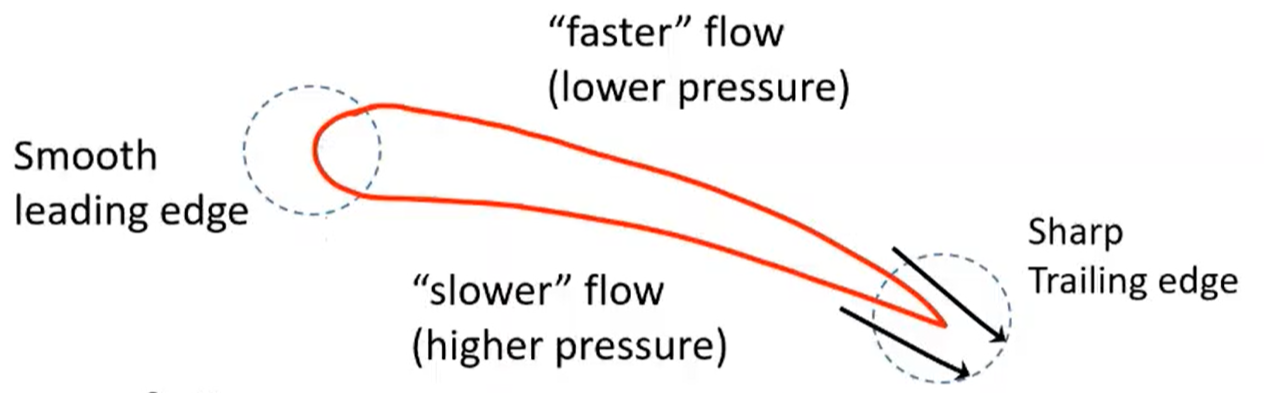
\includegraphics[width = 0.9 \textwidth]{./img/diagram30.png}
    \caption{Diagram of a subsonic aerefoil with the relevant pressures around it}
\end{figure}
For a subsonic aerefoil, the pressure around it varies continuously.
\subsection{Supersonic Aerofoil}
\begin{figure}[H]
    \centering
    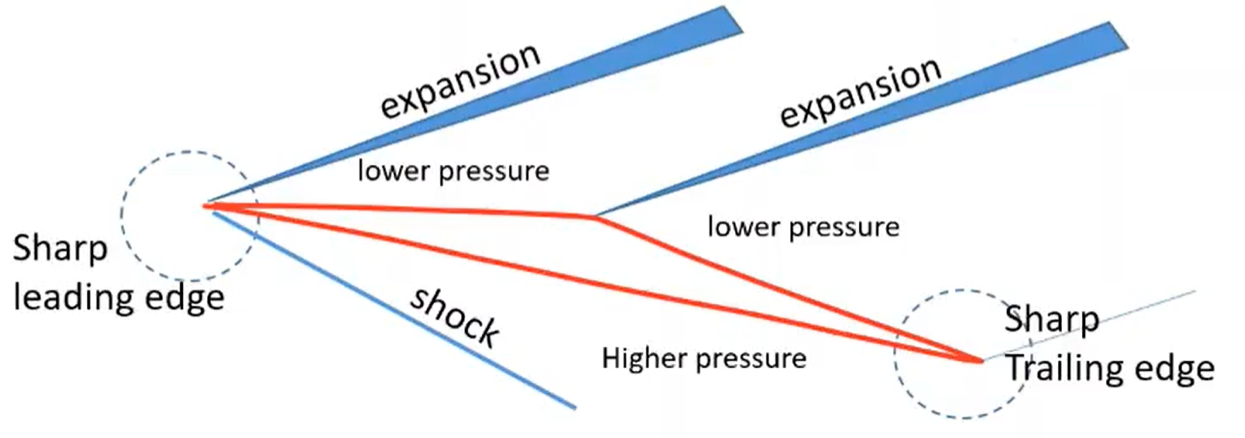
\includegraphics[width = 0.9 \textwidth]{./img/diagram31.png}
    \caption{Diagram of a supersonic aerefoil with the relevant pressures around it}
\end{figure}
For a supersonic aerefoil, the pressure around it is constant in different regions.
\section{Nonlinear Analysis}
We consider the case of a flat plate and examine the forces on it.
\begin{figure}[H]
    \centering
    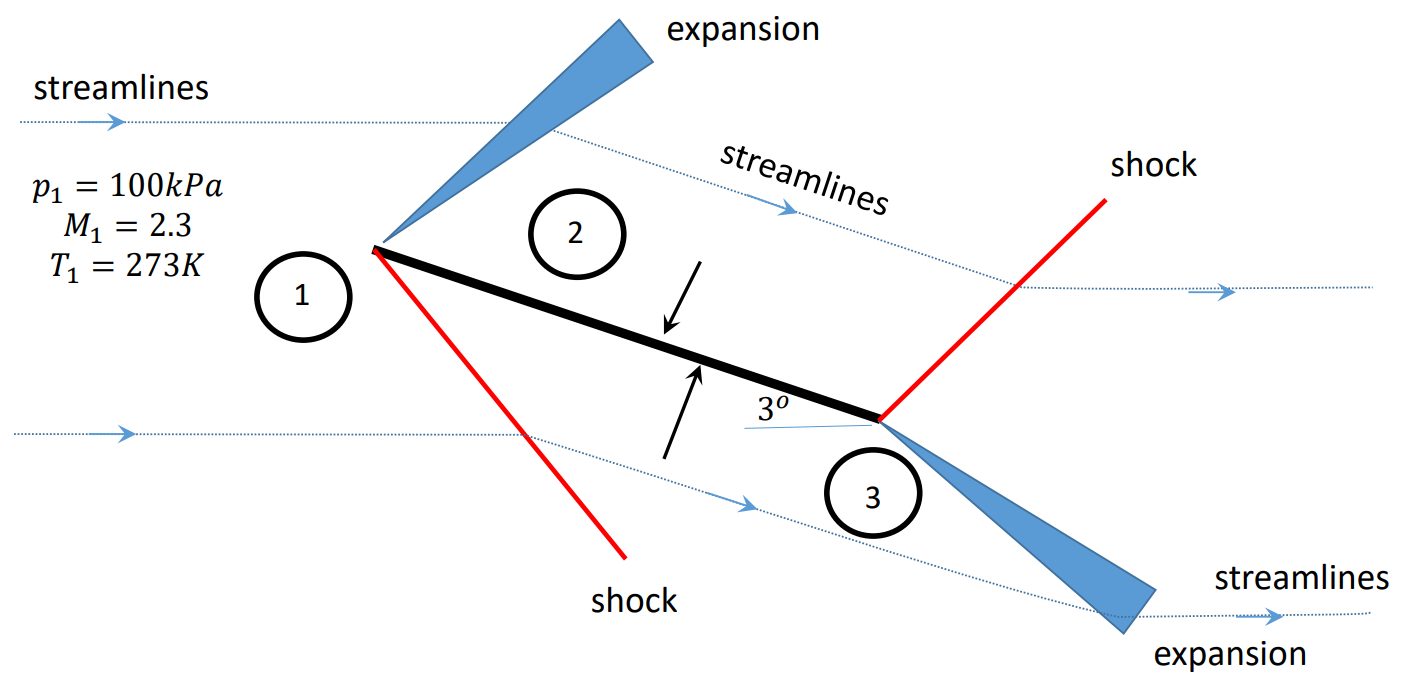
\includegraphics[width = 0.9 \textwidth]{./img/diagram32.png}
    \caption{The diagram of a flat plate with the relevant regions indicated}
\end{figure}
The initial conditions are:
\begin{gather}
    p_1 = 100\si{\kilo\pascal} \\[5pt]
    M_1 = 2.3 \\[5pt]
    T_1 = 273\si{\kelvin}
\end{gather}
\subsection{Use Shock Charts from Region 1 to Region 3}
The following results are obtained:
\begin{gather}
    \frac{p_3}{p_1} = 1.2
\end{gather}
Hence, the pressure in region 2 is calculated as:
\begin{gather}
    p_3 = 1.2\cdot 100 = 120\si{\kilo\pascal}
\end{gather}
\subsection{Use Expansion Charts for Region 1 to Region 2}
The following results are obtained:
\begin{gather}
    M_2 = 2.4 \\[5pt]
    \frac{p_2}{p_0} = 0.068 \\[5pt]
    \frac{p_1}{p_0} = 0.079
\end{gather}
Hence, the pressure in region 2 is calculated as:
\begin{gather}
    \frac{p_2}{p_1} = \frac{p_2}{p_0}\cdot \frac{p_0}{p_1} = 0.861 \\[5pt]
    \therefore p_2 = 0.861\cdot 100 = 86.1\si{\kilo\pascal}
\end{gather}
\subsection{Force Calculation}
The total force (per unit length) is:
\begin{gather}
    F_N = (p_3-p_2)L \\[5pt]
    = ((120-86.1)\cdot 10^3 \si{\pascal}) \cdot 1 \\[5pt]
    = (34\cdot 10^3\si{\pascal})\cdot 1
    = 34\si{\kilo\newton\per\metre}
\end{gather}
\subsection{Lift and Drag Coefficients}
\begin{figure}[H]
    \centering
    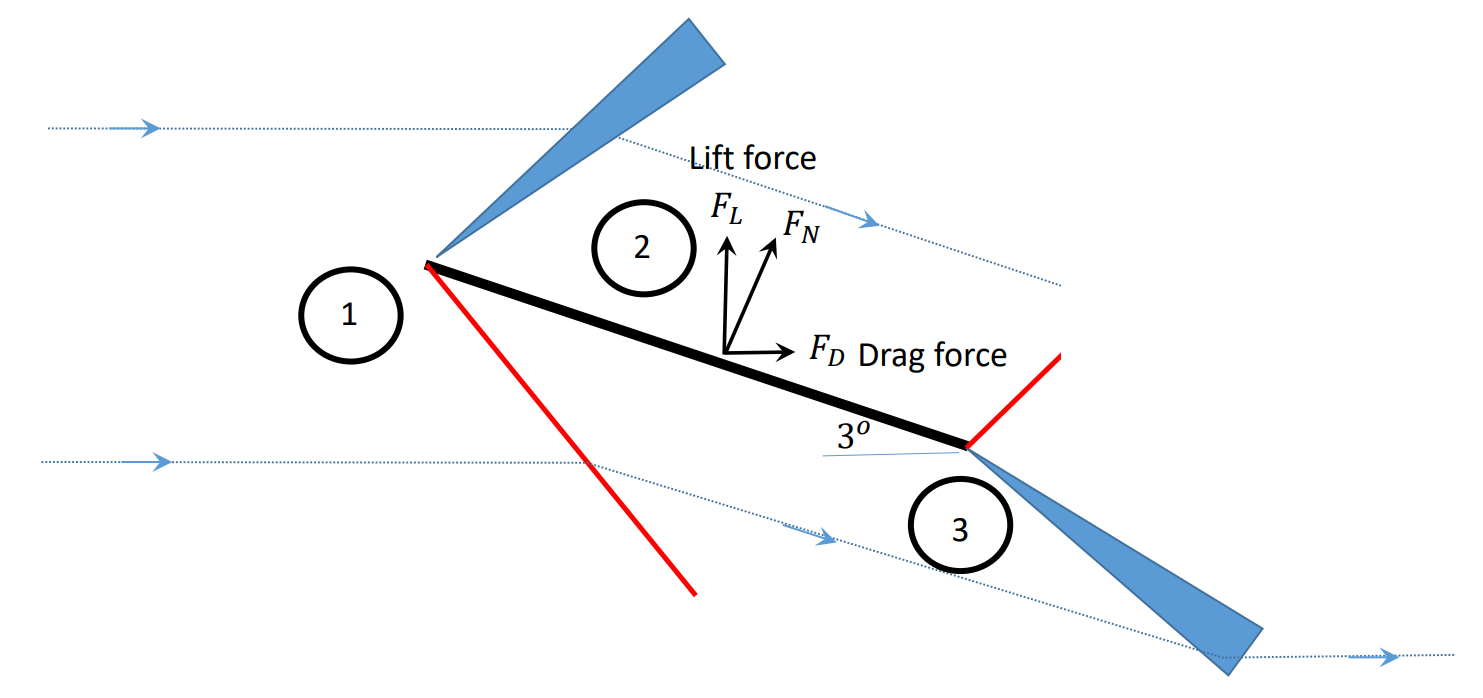
\includegraphics[width = 0.95 \textwidth]{./img/diagram33.png}
    \caption{The diagram of a flat plate with the lift and drag coefficients shown}
\end{figure}
Using:
\begin{gather}
    R = 287\si{\joule\per\kilogram\per\kelvin} \ \ \ \ \ \& \ \ \ \ \
    \gamma = 1.4
\end{gather}
The air speed is calculated as:
\begin{gather}
    u_1 = c_1 M_1 \\[5pt]
    c_1 = \sqrt{\gamma R T_1} \\[5pt]
    u_1 = \sqrt{\gamma R T_1} \cdot M_1 = \sqrt{1.4\cdot 287\cdot 273}\cdot 2.3 = 762 \si{\metre\per\second}
\end{gather}
The drag and lift forces are defined by:
\begin{gather}
    F_D = F_N \sin\alpha \\[5pt]
    F_L = F_N \cos\alpha
\end{gather}
The lift and drag coefficients are:
\begin{gather}
    c_D = \frac{F_D}{\dfrac{1}{2}\rho_1 u_1^2 L} \ \ \ \ \ \& \ \ \ \ \
    c_L = \frac{F_L}{\dfrac{1}{2}\rho_1 u_1^2 L}
\end{gather}
Substituting in the values yields:
\begin{gather}
    c_D = 0.0046 \\[5pt]
    c_L = 0.088
\end{gather}
Two observations can be made here:
\begin{enumerate}[noitemsep]
    \item It is quite hard to calculate
    \item $\dfrac{c_L}{c_D}>>1$
\end{enumerate}
\section{Linear Methods for Calculating Forces}
\begin{figure}[H]
    \centering
    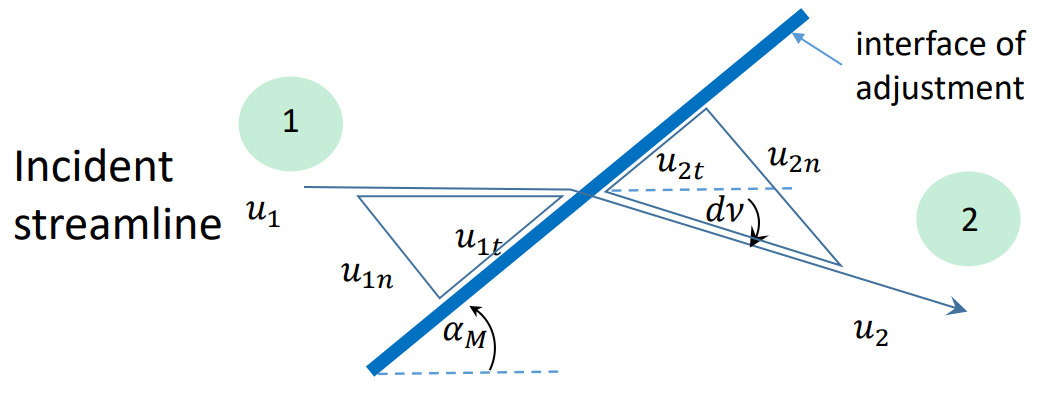
\includegraphics[width = 0.85 \textwidth]{./img/diagram34.png}
    \caption{}
\end{figure}
Conservation of momentum parallel to interface:
\begin{gather}
    u_1 \cos\alpha_M = u_2 \cos(\alpha_M + dv)
\end{gather}
From the double angle formula:
\begin{gather}
    \cos(\alpha_M + dv) \approx \cos\alpha_M - dv\sin\alpha_M
\end{gather}
Rearranging gives:
\begin{gather}
    \frac{\dif u}{u} = \frac{u_2-u_1}{u_2} = \frac{\sin\alpha_M}{\cos\alpha_M}dv
\end{gather}
We are trying to relate changes in pressure to the deflection angle.
All angles are relative to incident streamline and small so that $\abs{dv}<<1$, where:
\begin{itemize}[noitemsep]
    \item $\dif v$ - deflection or wedge angle
    \item $\alpha_M$ - shock wave angle
    \item $\sin\alpha_M = \dfrac{1}{M_1}$
\end{itemize}
To this linear approximation, a shock = - expansion.
\\\\
From the normal momentum equation:
\begin{gather}
    \rho_1 u_{1n} (u_{2n}-u_{1n}) = -(p_2-p_1)
\end{gather}
or
\begin{gather}
    \rho_1 u_1 \sin\alpha_M (u_2\sin(\alpha_M + \dif v)-u_1\sin\alpha_M) = -(p_2-p_1)
\end{gather}
Rearranging gives:
\begin{gather}
    \frac{p_2-p_1}{\dfrac{1}{2}\rho_1 u_1^2} = -\frac{2\sin\alpha_M}{u_1}(u_2(\sin\alpha_M + \cos\alpha_M \dif v) - u_1\sin\alpha_M) \\[5pt]
    = -\frac{2\sin\alpha_M}{u_1} \left(u_2 \dif v \frac{\sin^2 \alpha_M}{\cos\alpha_M} + u_2\cos\alpha_M \dif v\right) \\[5pt]
    \therefore \frac{p_2-p_1}{\dfrac{1}{2}\rho_1 u_1^2} = -\frac{2\sin\alpha_M}{\cos \alpha_M} \dif v \frac{u_2}{u_1} \approx -\frac{2\dif v}{\sqrt{M_1^2-1}}
\end{gather}
This is known as the linear model for small changes where $u_1$ and $M_1$ do not change.
\section{Example: Nonlinear Calculation}
We consider the case of a flat plate and examine the forces on it:
\begin{figure}[H]
    \centering
    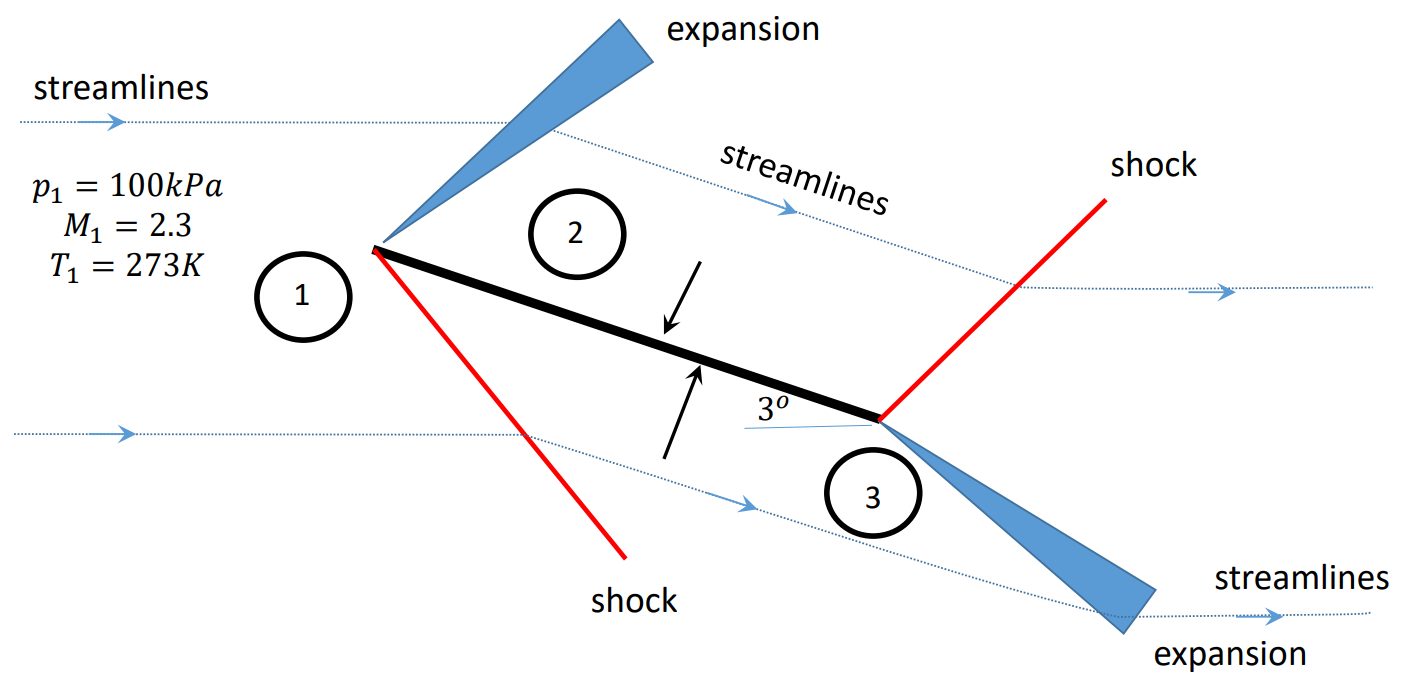
\includegraphics[width = 0.9 \textwidth]{./img/diagram32.png}
    \caption{The diagram of a flat plate with the relevant regions indicated}
\end{figure}
In applying this technique we need to make sure that we understand when a shock or expansion occurs. This tells us the sign of the pressure change.
\begin{gather}
    \frac{p_2-p_1}{\dfrac{1}{2}\rho_1 u_1^2} \approx -\frac{2\alpha}{\sqrt{M_1^2-1}} \\[5pt]
    \frac{p_3-p_1}{\dfrac{1}{2}\rho_1 u_1^2} \approx -\frac{2\alpha}{\sqrt{M_1^2-1}}
\end{gather}
\subsection{Lift and Drag Coefficients}
The normal force per unit length is calculated as:
\begin{gather}
    F_N = (p_3-p_2)L \\[5pt]
    = \frac{\dfrac{1}{2}\rho_1 u_1^2\left((2\alpha)-(-2\alpha)\right)L}{\sqrt{M_1^2-1}}
\end{gather}
The lift and drag coefficients are:
\begin{gather}
    c_D = \frac{F_N\sin\alpha}{\dfrac{1}{2}\rho_1 u_1^2 L} = \frac{\frac{\frac{1}{2}\rho_1 u_1^2\left((2\alpha)-(-2\alpha)\right)L}{\sqrt{M_1^2-1}}\sin\alpha}{\frac{1}{2}\rho_1 u_1^2 L} = \frac{4\alpha\sin\alpha}{\sqrt{M_1^2-1}} = 0.0059 \ \text{(Nonlinear 0.0048)} \\[5pt]
    c_L = \frac{F_N\cos\alpha}{\dfrac{1}{2}\rho_1 u_1^2 L} = \frac{\frac{\frac{1}{2}\rho_1 u_1^2\left((2\alpha)-(-2\alpha)\right)L}{\sqrt{M_1^2-1}}\cos\alpha}{\frac{1}{2}\rho_1 u_1^2 L} = \frac{4\alpha\cos\alpha}{\sqrt{M_1^2-1}} = 0.1 \ \text{(Nonlinear 0.092)}
\end{gather}
\section{Linear Calculation for More Complicated Geometry}
\begin{figure}[H]
    \centering
    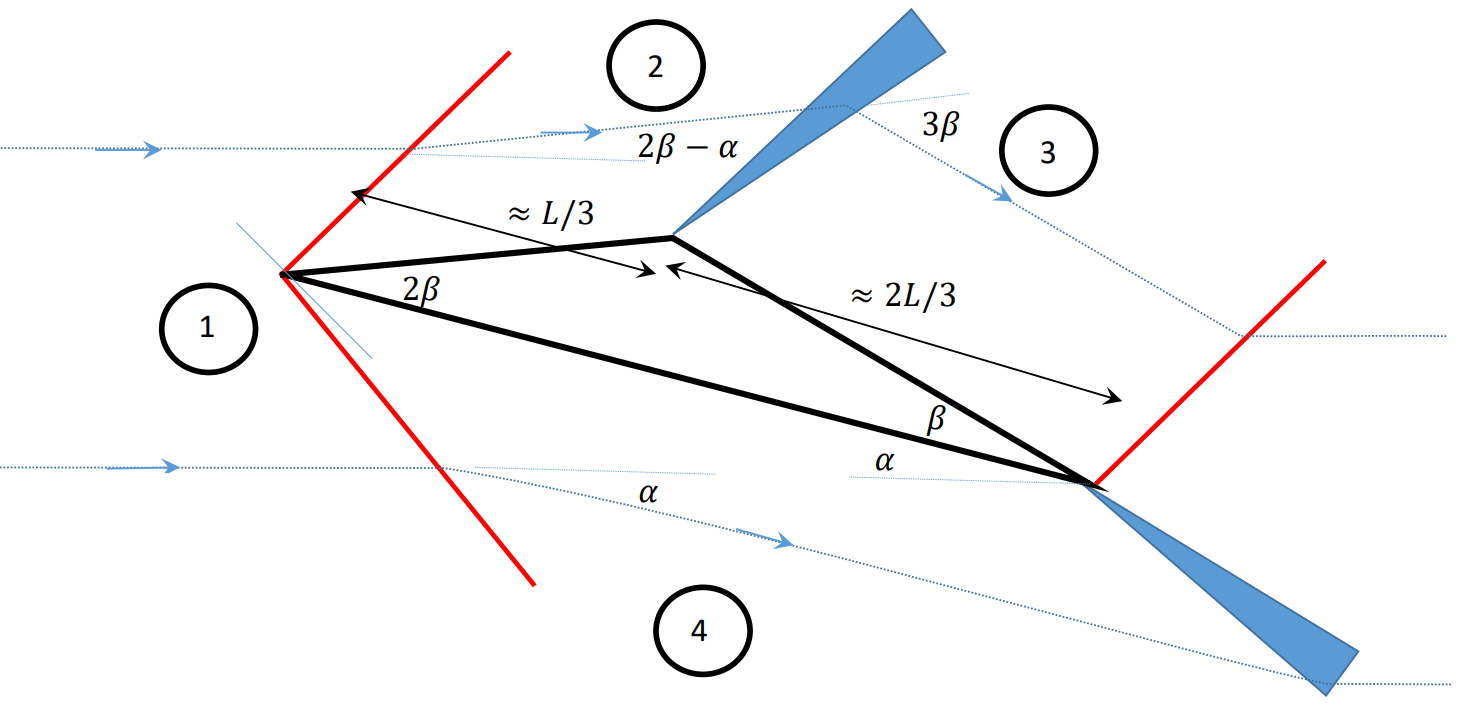
\includegraphics[width = 0.9 \textwidth]{./img/diagram35.png}
    \caption{The diagram for a more complicated geometry}
\end{figure}
To simplify the analysis, define:
\begin{gather}
    A = \frac{\dfrac{1}{2}\rho_1 u_1^2}{\sqrt{M_1^2-1}}
\end{gather}
Techniques for solution:
\begin{enumerate}[noitemsep]
    \item Draw a large figure
    \item Calculate the deflection angles
    \item Calculate the pressure differences between the different regions
\end{enumerate}
Pressures in each region:
\begin{gather}
    p_2-p_1 = 2(2\beta-\alpha)A \\[5pt]
    p_3-p_2 = -6\beta A \\[5pt]
    p_4-p_1 = 2\alpha A
\end{gather}
The second equation can be written as:
\begin{gather}
    p_3-p_1 = -(2\alpha+2\beta)
\end{gather}
The lift force is calculated as:
\begin{gather}
    F_L = p_4L\cos\alpha - p_2\frac{L}{3}\cos(2\beta-\alpha) - p_3\frac{2L}{3}\cos(\alpha+\beta)
\end{gather}
Through small angle approximation:
\begin{gather}
    F_L = p_4L - p_2\frac{L}{3} - p_3\frac{2L}{3} \\[5pt]
    \approx \left( 2\alpha - \frac{2}{3}(2\beta-\alpha) + \frac{2}{3}(2\alpha+2\beta) \right) AL
\end{gather}
The drag force is calculated as:
\begin{gather}
    F_D = p_4L\sin\alpha + p_2\frac{L}{3}\sin(2\beta-\alpha) - p_3\frac{2L}{3}\sin(\alpha+\beta)
\end{gather}
Through small angle approximation:
\begin{gather}
    F_D = p_4L\alpha + p_2\frac{L}{3}(2\beta-\alpha) - p_3\frac{2L}{3}(\alpha+\beta) \\[5pt]
    \approx \left( 2(\alpha)(\alpha) + \frac{2}{3}(2\beta-\alpha)(2\beta-\alpha) + \frac{2}{3}(2\alpha+2\beta)(\alpha+\beta) \right) AL \\[5pt]
    = \left( 2\alpha^2 + \frac{2}{3}(4\beta^2-4\beta\alpha+\alpha^2) + \frac{4}{3}(\alpha^2+2\beta\alpha+\beta^2) \right) AL \\[5pt]
    = (4\alpha^2+4\beta^2)AL
\end{gather}
The lift and drag coefficients are:
\begin{gather}
    c_L = \frac{F_L}{\dfrac{1}{2}\rho_1 u_1^2 L} = \frac{4\alpha}{\sqrt{M_1^2-1}} \\[5pt]
    c_D = \frac{F_D}{\dfrac{1}{2}\rho_1 u_1^2 L} = \frac{4(\alpha^2+\beta^2)}{\sqrt{M_1^2-1}}
\end{gather}
The solution reduces to flat plate case when $\beta = 0$.
\section{Lift Coefficient Variation with Mach Number}
\begin{figure}[H]
    \centering
    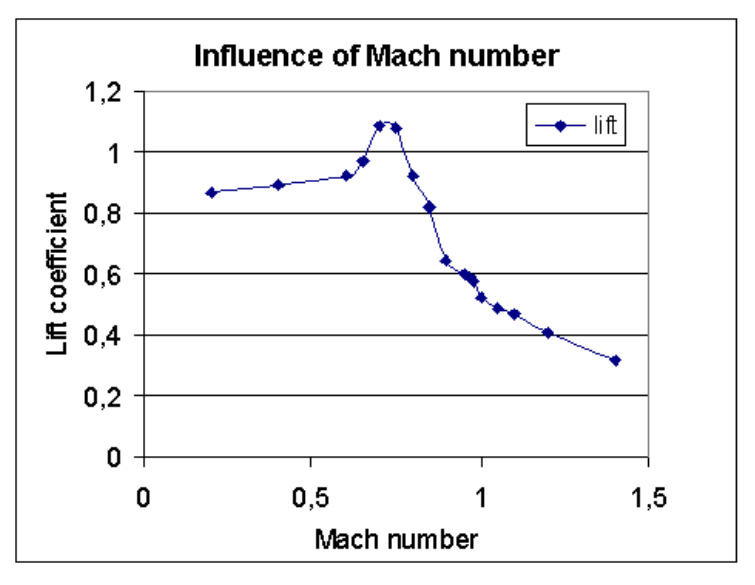
\includegraphics[width = 0.65 \textwidth]{./img/diagram36.png}
    \caption{Lift coefficient variation with Mach number}
\end{figure}
For low Mach number:
\begin{gather}
    c_D \sim constant \\[5pt]
    c_L \sim 2\pi\alpha
\end{gather}
For high Mach number:
\begin{gather}
    c_D \sim \frac{4\alpha^2}{\sqrt{M_1^2-1}} \\[5pt]
    c_L \sim \frac{4\alpha}{\sqrt{M_1^2-1}}
\end{gather}